\section{A description of \acs{EsPy}}

\subsection{Why \textsc{Python}?}
There a number of reasons why \textsc{Python} was the chosen programming
language for \ac{EsPy}:
\begin{itemize}
    \item It has a large user-base, particularly within the scientific
        community.
    \item The \textsc{SciPy} ecosystem\cite{Virtanen2020}, including the packages
        \textsc{NumPy}\cite{Harris2020} and
        \textsc{Matplotlib}\cite{Hunter2007} is a powerful tool which enables
        high-performance scientific computation an visualisation in
        \textsc{Python}, despite the language's reputation for slow speed.
    \item Being a scripting language with user-friendly syntax makes
        \textsc{Python} ideal for exploring datasets in a step-by-step fashion.
        This is useful in the context of \ac{EsPy}, as a user will want to
        (i) inspect and pre-process the data of interest,
        (ii) determine the regions they wish to estimate and set up the
        routine,
        (iii) output and inspect the result.
        This can be achieved easily by ``hacking'' and re-running
        \textsc{Python} scripts or by using ``notebook'' environments, such as
        \textsc{Jupyter}.
    \item It is free and open-source, as opposed to well-known scientific
        computing platforms such as \textsc{Matlab} and \textsc{Mathematica}.
    \item \textsc{Python} supports sophisticated object-oriented programming
        features, including multiple levels of inheritance. This is exploited in
        \ac{EsPy} in order to create numerous objects designed with specific
        \ac{NMR} data types in mind.
\end{itemize}

Probably the largest disadvantage in using \textsc{Python} is its slow performance on
account of it being an interpreted, dynamically typed language which relies on
garbage collection for memory management. While \textsc{NumPy} provides
interfaces to run fast computations with pre-compiled C-code, a significant
performance benefit would likely be realised if a low-level compiled language
like C, C++, or \textsc{Rust} were used instead (this is discussed more in
\cref{sec:future-work}). While this may be so, the
development time in writing programs with these lower-level languages is
typically a lot greater than with a language with a higher level of abstraction
like \textsc{Python}.

\subsection{Estimator objects}
\begin{figure}
    \centering
    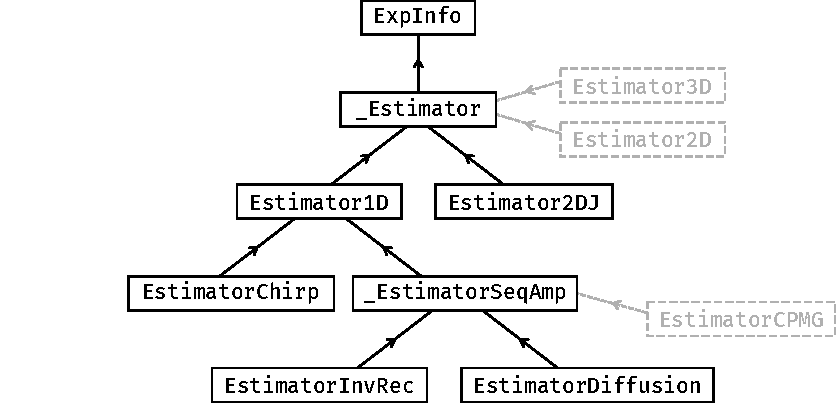
\includegraphics{inheritance_tree/inheritance_tree.pdf}
    \caption[
        Inheritance tree for estimation classes in the \acs{EsPy} package.
    ]{
        Inheritance tree for estimation classes in the \acs{EsPy} package.
        Arrows are directed from child classes to the parent class they
        directly inherit from. Classes in grey are objects that could be added
        to the \ac{API} in the future.
    }
    \label{fig:inheritance}
\end{figure}
The fundamental user-facing objects (or classes) that \ac{EsPy} provides are
\emph{estimators}.
Instances of these estimator objects contain relevant
\emph{attributes} (the \ac{FID}, experiment parameters including the sweep
width, transmitter offset etc), as well as \emph{methods} which perform useful
routines like estimation and result figure generation.
Thanks to \textsc{Python}'s support for multiple levels of inheritance, it is
possible to build numerous objects with certain shared attributes and methods,
but which also possess bespoke features that are solely of relevance to
the type of \ac{NMR} data being considered. As an example, only the
\texttt{Estimator2DJ} object possesses a method called \texttt{cupid\_spectrum},
which returns the \ac{FT} of the \ang{-45} signal.
\Cref{fig:inheritance} provides an \emph{inheritance
diagram} for the different estimator classes in \ac{EsPy}. Basic overviews of
each class are as follows:
\begin{itemize}
    \item \textbf{\textbf{\texttt{ExpInfo}}}: Stores parameters used in a particular \ac{NMR}
        experiment. \texttt{ExpInfo} also has methods for the generation of the
        timepoints/chemical shifts sampled based on these parameters, and for
        producing synthetic \acp{FID}.
    \item \textbf{\texttt{\_Estimator}}: Also possesses the \ac{NMR} data as an
        attribute on top of the experiment information. This class is
        designed to contain the functionality which can be generalised across
        all \ac{NMR} data types supported by \ac{EsPy}. It does not
        possess all the features necessary to useful as a standalone object,
        and as such the user is not permitted to use it directly (such an
        object is often referred to as an \emph{abstract class}). For child
        classes of \texttt{\_Estimator}, the main feature that requires methods
        to be defined is the means by which the data is imported (experimental
        data) or generated (simulated data).
    \item \textbf{\texttt{Estimator1D}}: Conventional \ac{1D} datasets are
        analysed using this class (\cref{sec:evaluation}).
    \item \textbf{\texttt{\_EstimatorSeqAmp}}: An abstract class
        which enables the estimation of sequential \ac{1D} datasets
        (\cref{sec:seq}). Analysis of the dataset varies depending on
        the type of experiment considered, such as the function used for
        fitting amplitudes (\cref{tab:seq-equations}), and the means by
        which that data should be imported/generated. As such, this is not
        designed for direct use; one of the classes which inherit it should be
        used instead. \texttt{\_EstimatorSeqAmp} stores a number of
        \texttt{Estimator1D} objects, with each object containing one of the
        \acp{FID} in the sequential dataset. Estimation simply comprises
        looping through these estimators, giving the parameter estimate of the
        previous estimator to next as its initial guess.
    \item \textbf{\texttt{EstimatorInvRec}}: For the estimation of inversion
        recovery ($T_1$) datasets.
    \item \textbf{\texttt{EstimatorDiffusion}}: For the estimation of
        diffusion datasets.
    \item \textbf{\texttt{EstimatorChirp}}: For the estimation of \acp{FID}
        acquired using single-chirp excitation (\cref{sec:bbqchili}).
    \item \textbf{\texttt{Estimator2DJ}}: For the estimation of \ac{2DJ} data.
        This class also provides features to generate pure shift spectra and
        assign multiplet structures using \ac{CUPID} (\cref{chap:cupid}).
\end{itemize}

Other estimator objects which are yet to be implemented, but are potential
future additions to the package are also depicted in the inheritance diagram.
\texttt{EstimatorCPMG} would be for the consideration of \ac{CPMG} datasets,
which enable the determination of $T_2$ times.
\texttt{Estimator2D} and \texttt{Estimator3D} would be
for the estimation of datasets comprising sets of \ac{2D} or \ac{3D} amplitude-
or phase-modulated \acp{FID}, respectively. A discussion of the feasibility of
implementing these is given in \cref{sec:future-work}.
